% !TEX root = cha-approach.tex
\documentclass[../../main.tex]{subfiles}

\begin{document}

\section{Relationship Representation}

After placing the classes, the relationships between them are represented as paths. Drawing a separate path for every relationship would quickly lead to a cluttered visualization~\citebibliography{Ball1996a}. Therefore, relationships are merged into a single path when they have the same destination and the same relationship type.

For example, if classes B, C, and D are all subclasses of class A, their relationships can be represented by a single path from B, C, and D to A. Similarly, if classes B and C both call a method of class E, these relationships are represented by a single path from B and C to E. A conceptual example of this merging process is shown in \figref{fig:relationship-merging}.

\begin{figure}[ht]
    \centering
    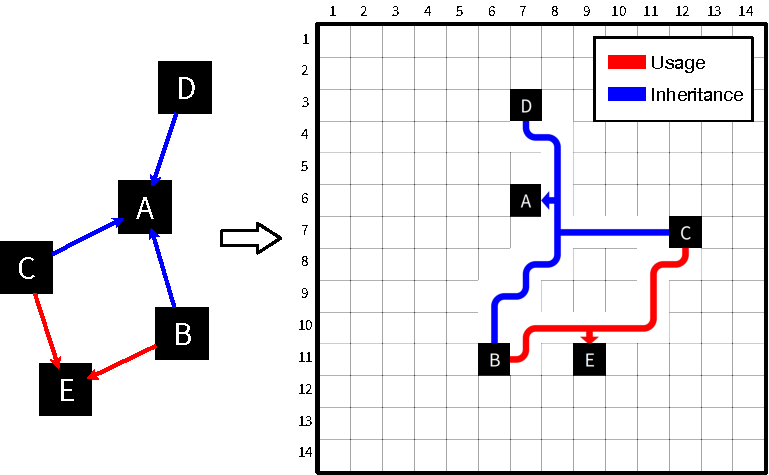
\includegraphics[width=\linewidth]{figures/approach/relationship_merging.pdf}
    \caption{Conceptual representation of path merging.}
    \label{fig:relationship-merging}
\end{figure}

Different relationship types are represented using different colors. For example, hierarchy relationships are shown in blue, while method calls are shown in red. This allows the type of a relationship to be identified directly from the visualization.

Path merging also reduces the total number of paths that WFC has to generate, which can make it easier for WFC to find a valid solution. Moreover, merging paths also reduces the number of border cells that a class needs to expose. Nevertheless, we keep the footprint of the class proportional to the \emph{overall non-merged} number of connections as this serves as an explicit visual encoding to highlight highly connected classes.

Each merged path is assigned a unique path ID based on the IDs of its source classes, its destination class, and its relationship type. The path ID is used to enforce the global connectivity constraint using only the local ones of WFC.

The path ID is embedded in the border cells of the corresponding classes and propagated through the grid during WFC. A path can therefore only start from and terminate at cells containing its ID. This ensures that paths connect the intended classes and prevents them from connecting unrelated classes. When multiple relationships are merged into the same path, they share the same path ID, ensuring that they are represented as a single path.

\end{document}